\documentclass{beamer}
\usepackage{beamerthemesplit}
\usepackage{graphics}
\logo{
\includegraphics[height=1cm]{psi_logo_white.png}}
\usetheme{Pittsburgh}
\usecolortheme{dove}
\beamertemplatenavigationsymbolsempty
\setbeamertemplate{footline}[frame number]
\definecolor{myback}{RGB}{175,238,238}
\setbeamercolor{structure}{bg=myback}
\usepackage[T1]{fontenc}
\newcommand{\changefont}[3] {
\fontfamily{#1} \fontseries{#2} \fontshape{#3} \selectfont}


\title{NeXus Rules and Details }
\author{Mark K\"onnecke }
\institute{Paul Scherrer Institute\\Switzerland }
\date{\today} 

\begin{document}

\begin{frame}
\titlepage
\end{frame}

\begin{frame}
\frametitle{Overview}
\begin{itemize}
\item NeXus coordinate systems 
\item File structural rules
\item Rules for storing data items
\item Rules for special applications
\item Special NeXus groups
\end{itemize}
\end{frame}

\begin{frame} \frametitle{McStas Coordinate System }
\begin{figure}[!ht]
\resizebox{7cm}{5cm}{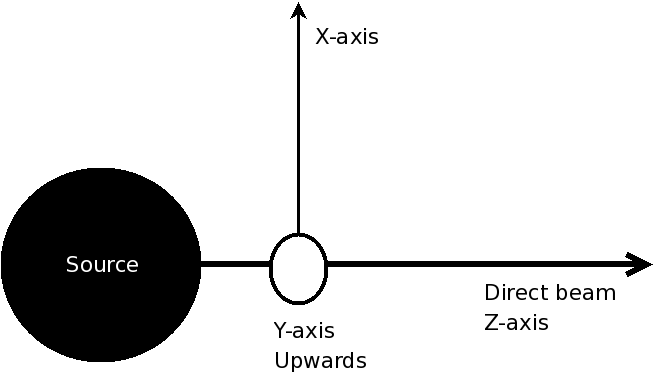
\includegraphics[width=0.95\textwidth]{mcstas.png}}\end{figure}
\end{frame}

\begin{frame} \frametitle{NeXus Simple Coordinate System }
\begin{figure}[!ht]
\resizebox{7cm}{5cm}{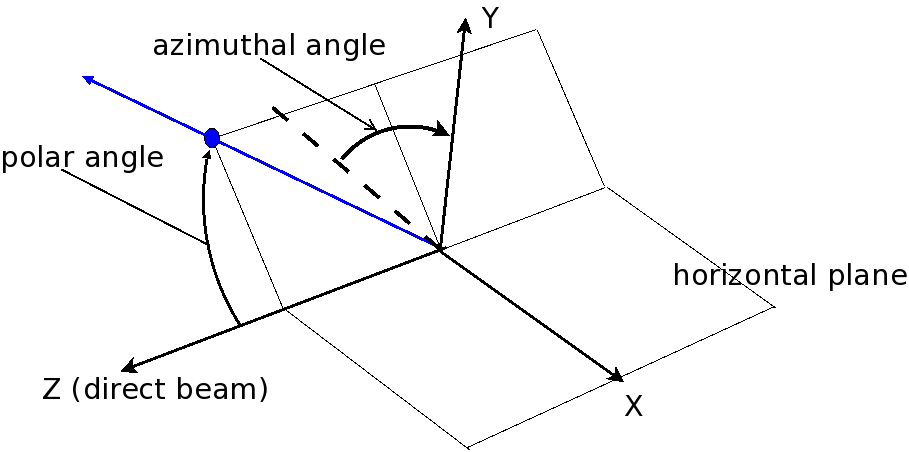
\includegraphics[width=0.95\textwidth]{polplane.png}}\end{figure}
\end{frame}


\begin{frame} \frametitle{Polar\_angle }
Polar angle is always relative to the previous component 
\begin{figure}[!ht]
\resizebox{7cm}{5cm}{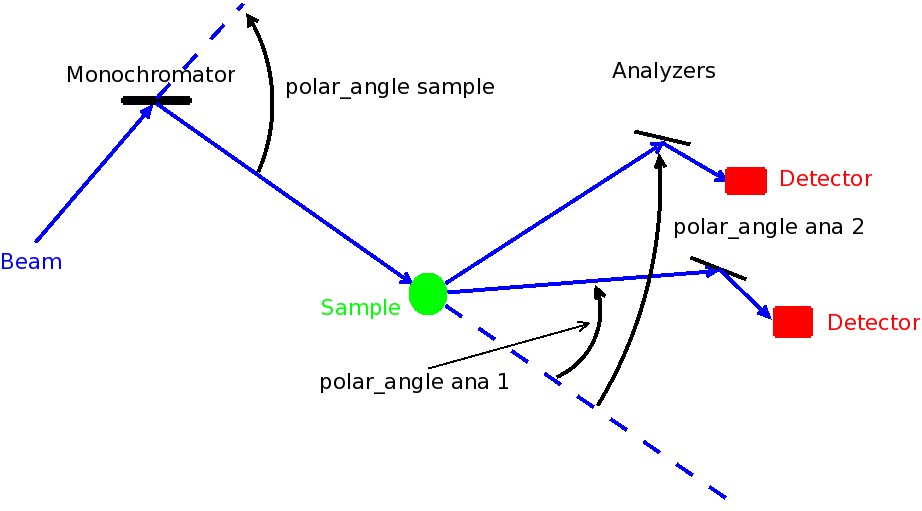
\includegraphics[width=0.95\textwidth]{polarangle.png}}\end{figure}
\end{frame}


\begin{frame} \frametitle{CIF like Coordinates (Proposed)}
\begin{itemize}
\item Additional fields in base classes: transform, x\_translation, y\_translation, z\_translation, 
  aequatorial\_angle
\item $Pcurrent = op1*op2*op3*...*P0$
\item transform is a komma separated list of axis to apply to the component to get into position. 
\item Additional data attributes: 
\begin{itemize}
\item type: translation or rotation
\item vector: rotation or translation axis
\item offset: offset to center of component
\end{itemize}
\item Use this for documentation or arbitrary axis specifications
\end{itemize}
\end{frame}

\begin{frame} \frametitle{NeXus Default Coordinates (CIF like)}
\begin{itemize}
\item polar\_angle: type= rotation, vector= 0,1,0, offset= 0, 0, -distance
\item azimuthal\_angle: type=rotation, vector 0,0,1
\item transform: azimuthal\_angle, polar\_angle
\end{itemize}
\end{frame}


\begin{frame} \frametitle{NXgeometry}
\begin{itemize}
\item Special group structure which can be added to any base class
\end{itemize}
\begin{tabbing}
\hspace*{1cm} \= \hspace*{1cm} \= \hspace*{1cm} \= \hspace*{1cm} \= \hspace*{1cm} \= \hspace*{1cm}\= \kill
geometry:NXgeometry \\
 \>translation:NXtranslation \\
\> \>translation[3]\\
\>shape:NXshape\\
\> \>shape: nxbox|nxcylinder|nxsphere,
\> \>size[]\\
\>orientation:NXorientation\\
\> \>vector[3]\\
\end{tabbing}
\end{frame}


\begin{frame}
\frametitle{NeXus General Rules}
\begin{itemize}
\item NeXus reserves the prefix NX for group names.  
\item Store as much as possible
\item A NeXus file has one to many NXentry groups 
\item There are two types of entries: raw data and processed data
\item Multiple different techniques in one file go into separate entries
\item If there is only one entry, the preferred name is entry, else entry1, entry2... entryn
\item If an entry conforms to an application definition, the application definitions must be stated in the 
 entries definition field.
\end{itemize}
\end{frame}

\begin{frame} \frametitle{NeXus Raw Data File Structure}
\begin{tabbing}
\hspace*{1cm} \= \hspace*{1cm} \= \hspace*{1cm} \= \hspace*{1cm} \= \hspace*{1cm} \= \hspace*{1cm}\= \kill
entry:NXentry \\
 \>sample:NXsample \\
\\
 \>instrument:NXinstrument\\
 \> \> source:NXsource\\
 \> \> velocity\_selector:NXvelocity\_selector\\
 \> \> detector:NXdetector \\
 \> \> \>data[xsize,ysize], signal=1 (1)\\
 \>control:NXmonitor\\
 \> \>data\\
 \>data:NXdata\\
 \> \> link to (1)\\
\end{tabbing}
\end{frame}

\begin{frame} \frametitle{NeXus Processed Data File Structure}
\begin{tabbing}
\hspace*{1cm} \= \hspace*{1cm} \= \hspace*{1cm} \= \hspace*{1cm} \= \hspace*{1cm} \= \hspace*{1cm}\= \kill
entry:NXentry \\
 \>sample:NXsample \\
 \>processing\_name:NXprocess\\
 \> \>program \\
 \> \>version \\
 \> \>parameters:NXparameter \\
 \> \> \>raw\_file \\
 \>data:NXdata\\
 \> \> data[nx,ny,nz], signal=1\\
\end{tabbing}
\end{frame}


\begin{frame}
\frametitle{Rules for Storing Data Items}
\begin{itemize}
\item Store physical values
\item Use NeXus components and dictionary names
\item Missing names will be quickly accepted by the NIAC
\item Names: full words separated by \_
\item Specify units in same format as used by UDunits
\item Application definitions may restrict units
\end{itemize}
\end{frame}

\begin{frame}
\frametitle{Scaled Data (Proposed)}
\begin{itemize}
\item NeXus {\em STRONGLY} prefers plain data in C storage order
\item Additional  attributes: linearity, offset, scaling, direction, precedence
\item Same meaning as in imageCIF
\item linearity:
\begin{itemize}
\item offset: Vtrue = Vraw + offset
\item scaling: Vtrue = Vraw * scaling
\item scaling\_offset: Vtrue (Vraw/scaling) + offset
\item sqrt\_scaled: $Vtrue = (Vraw/scaling)^2$
\item logarithmic\_scaled: $Vtrue = 10^(Vraw/scaling)$
\end{itemize}
\item direction allows to select between increasing and decreasing indices
\item precedence determines storage order
\end{itemize}
\end{frame}


\begin{frame} \frametitle{Associating Axis and Data}
\begin{itemize}
\item Data and axis live in the same NXgroup
\end{itemize}
\begin{tabbing}
\hspace*{1cm} \= \hspace*{1cm} \= \hspace*{1cm} \= \hspace*{1cm} \= \hspace*{1cm} \= \hspace*{1cm}\= \kill
entry:NXentry \\
 \>data:NXdata\\
 \> \> data[nx,ny,nz], signal=1\\
 \> \> x\_axis[nx], axis=1\\
 \> \> y\_axis[ny], axis=2\\
 \> \> z\_axis[nz], axis=3\\
\end{tabbing}
\end{frame}

\begin{frame} \frametitle{Multiple Axis}
\begin{tabbing}
\hspace*{1cm} \= \hspace*{1cm} \= \hspace*{1cm} \= \hspace*{1cm} \= \hspace*{1cm} \= \hspace*{1cm}\= \kill
entry:NXentry \\
 \>data:NXdata\\
 \> \> data[nx,ny,nz], signal=1\\
 \> \> x\_axis[nx], axis=1, primary=1\\
 \> \> alternate\_x\_axis[nx], axis=1\\
 \> \> y\_axis[ny], axis=2\\
 \> \> z\_axis[nz], axis=3\\
\end{tabbing}
\end{frame}

\begin{frame} \frametitle{Associating Axis and Data, Method 2}
\begin{tabbing}
\hspace*{1cm} \= \hspace*{1cm} \= \hspace*{1cm} \= \hspace*{1cm} \= \hspace*{1cm} \= \hspace*{1cm}\= \kill
entry:NXentry \\
 \>data:NXdata\\
 \> \> data[nx,ny,nz], signal=1, axes=x\_axis,y\_axis,z\_axis\\
 \> \> x\_axis[nx]\\
 \> \> y\_axis[ny]\\
 \> \> z\_axis[nz]\\
\end{tabbing}
\end{frame}


\begin{frame}
\frametitle{Storing Detector Data}
\begin{itemize}
\item Preserve original dimensionality of detector, if possible
\item Time-of-flight becomes last dimension
\item Highly irregular detectors:
\end{itemize}
\begin{tabbing}
\hspace*{1cm} \= \hspace*{1cm} \= \hspace*{1cm} \= \hspace*{1cm} \= \hspace*{1cm} \= \hspace*{1cm}\= \kill
entry:NXentry \\
\>instrument:NXinstrument\\
\> \>detector:NXdetector\\
\>  \> \> data[ndet], signal=1\\
\> \> \> polar\_angle[ndet], axis=1\\
\> \> \> azimuthal\_angle[ndet]\\
\> \> \> distance[ndet]\\
\end{tabbing}
\end{frame}


\begin{frame}
\frametitle{Scans}
\begin{itemize}
\item Come in all shapes and sizes
\item Captured by rules:
\begin{itemize}
\item Store all varied parameters as arrays of length NP at the appropriate place in the NeXus 
 hierarchy
\item For multi detectors, NP, number of scan points is always the first dimension
\item In NXdata: create links to counts and varied variables
\end{itemize}
\end{itemize}
\end{frame}


\begin{frame}
\frametitle{Scan Example 1: rotating sample}

\begin{tabbing}
\hspace*{1cm} \= \hspace*{1cm} \= \hspace*{1cm} \= \hspace*{1cm} \= \hspace*{1cm} \= \hspace*{1cm}\= \kill
entry:NXentry \\
 \>sample:NXsample\\
 \> \> rotation\_angle[NP], axis=1 (1) \\
 \> instrument:NXinstrument\\
 \>  \>detector:NXdetector\\
 \>  \> \>data[NP],signal=1 (2)\\
 \>control:NXmonitor\\  
 \> \>data[NP]\\  
 \>data:NXdata\\
 \> \> link to (1)\\
 \> \> link to (2) \\
\end{tabbing}
\end{frame}

\begin{frame}
\frametitle{Scan Example 2: complex scan in Q}

\begin{tabbing}
\hspace*{1cm} \= \hspace*{1cm} \= \hspace*{1cm} \= \hspace*{1cm} \= \hspace*{1cm} \= \hspace*{1cm}\= \kill
entry:NXentry \\
 \>sample:NXsample\\
 \> \> rotation\_angle[NP], axis=1 (1) \\
 \> \> phi[NP], axis=1 (2) \\
 \> \> chi[NP], axis=1 (3) \\
 \> \> h[NP], axis=1 (4), primary=1 \\
 \> \> k[NP], axis=1 (5) \\
 \> \> l[NP], axis=1 (6) \\
 \> instrument:NXinstrument\\
 \>  \>detector:NXdetector\\
 \>  \> \>data[NP],signal=1 (7)\\
 \>  \> \>polar\_angle[NP],signal=1 (8)\\
 \>data:NXdata\\
 \> \> link to (1)\\
 \> \> link to (2) \\
 \> \> link to (...) \\
 \> \> link to (8) \\
\end{tabbing}
\end{frame}


\begin{frame}
\frametitle{Scan Example 3: sample rotation, area detector}
\begin{tabbing}
\hspace*{1cm} \= \hspace*{1cm} \= \hspace*{1cm} \= \hspace*{1cm} \= \hspace*{1cm} \= \hspace*{1cm}\= \kill
entry:NXentry \\
 \>sample:NXsample\\
 \> \> rotation\_angle[NP], axis=1 (1) \\
 \> instrument:NXinstrument\\
 \>  \>detector:NXdetector\\
 \>  \> \>data[NP,xsize,ysize],signal=1 (2)\\
 \>control:NXmonitor\\  
 \> \>data[NP]\\  
 \>data:NXdata\\
 \> \> link to (1)\\
 \> \> link to (2) \\
\end{tabbing}
\end{frame}


\begin{frame}
\frametitle{Rasterisation}
\begin{itemize}
\item This is rastering a sample at different wavelengths, positions etc. 
\item Same treatment as scans, NP replaced by NR number of raster points
\item For the common case of rastering on a 2D grid one can store [nx,ny,detdim]. Be aware, though, that 
 this causes problems if the rasterisation is aborted in mid operation. 
\end{itemize}
\end{frame}

\begin{frame}
\frametitle{NXlog}
\begin{tabbing}
\hspace*{1cm} \= \hspace*{1cm} \= \hspace*{1cm} \= \hspace*{1cm} \= \kill
name\_of\_logged\_value:NXlog \\
  \> time[], start \\
  \>value[]\\
  \>description\\
  \>minimum\_value\\
  \>maximum\_value\\
  \>average\_value\\
\end{tabbing}
\end{frame}


\begin{frame}
\frametitle{NXnote}
\begin{tabbing}
\hspace*{1cm} \= \hspace*{1cm} \= \hspace*{1cm} \= \hspace*{1cm} \= \kill
note:NXlog \\
  \>author \\
  \>type\\
  \>date\\
  \>description\\
  \>file\_name\\
  \>data, NX\_BINARY\\
\end{tabbing}
\end{frame}


\begin{frame}
\frametitle{All Base Classes}
\begin{tabular}{lll}
NXaperture & NXattenuator & NXbeam\_stop \\
NXbeam     & NXbending\_magnet & NXcharacterization \\
NXcollimator & NXcrystal & NXdata \\
NXdetector   & NXdisk\_chopper & NXentry \\
NXenvironment & NXevent\_data & NXfermi\_chopper \\
NXfilter & NXflipper & NXgeometry \\
NXguide & NXinsertion\_device & NXinstrument \\
NXlog & NXmirror & NXmoderator \\
NXmonitor & NXmonochromator & NXnote \\
NXorientation & NXparameters & NXpolarizer\\
NXprocess & NXsample & NXsensor \\
NXshape & NXsource & NXtranslation\\
NXuser & NXvelocity\_selector & \\
\end{tabular}
\end{frame}


\end{document}

\begin{frame}
\frametitle{}
\begin{itemize}
\item
\end{itemize}
\end{frame}


\begin{frame} \frametitle{Using Tabbing for Hierarchy}
\begin{tabbing}
\hspace*{1cm} \= \hspace*{1cm} \= \hspace*{1cm} \= \hspace*{1cm} \= \kill
entry:NXentry \\
 \>sample:NXsample \\
 \> \> rotation\_angle[NP], axis=1 (1) \\
\\
 \>instrument:NXinstrument\\
 \> \> detector:NXdetector \\
 \> \> \>data[NP], signal=1 (2)\\
 \>data:NXdata\\
 \> \> link to (1)\\
 \> \> link to (2)\\
\end{tabbing}
\end{frame}

